\chapter{Data processing}

\section{Imputation}

\subsection{Background}
Most relevant algorithms for time series classification do not accommodate missing values. Both the .csv data format utilized for storing the data and some internal data representations employed by sktime and sklearn for processing do not account for missing values. These missing values are represented as "NaN", which stands for "Not a Number". In this document, we will refer to these missing values as NaNs.

To address this issue, several methods can be employed:
\begin{itemize}
\item After collecting all the data, remove any columns containing NaNs. This approach results in data loss but ensures the accuracy of all remaining values, as it avoids estimation.
\item Limit algorithm usage to only those capable of handling NaNs. A considerable number of algorithms in sklearn and sktime can work in this manner, but it still imposes a constraint \cite*{Scikit-learn-imputation}.
\item Implement imputation of missing values, which entails using an algorithm to make an informed guess about a plausible value based on existing values in similar positions.
\item Perform dimensionality reduction on the data. Reduction algorithms like Singular Value Decomposition (SVD) are good for removing dummy data like NaNs.
\end{itemize}

Initially, the first method was effective for the project. This was due to the simulation being poorly configured and not subjected to significant stress. Additionally, there were insufficient time points collected and an inadequate number of instances generated. This meant that there were few opportunities for NaNs to appear in the collected data, so few columns had to be discarded. When the stress testing improved to be more stressful and more data points were gathered, significantly more NaNs appeared and quite a few columns would have to be discarded, inflicting significant data loss.
The second method was briefly considered, but since the project's primary goal was to compare multiple classification methods, this idea was quickly discarded.

Ultimately, imputation emerged as the most suitable solution. Imputation of univariate datasets is typically straightforward: Missing values are assigned the mean, median, or most frequent value for their respective column. Multivariate imputation is more challenging. The primary issue is that each column may exhibit significant variation between instances. Simply using a statistic about the entire column would dilute the data, thereby worsening the signal-to-noise ratio.
\section{Series length}
The data collection program that collects the Prometheus data and saves it as .csv files strives to obtain the same number of time points for each instance. This is achieved by using consistent timeframes and collection intervals. However, this is not always possible.

Factors such as the test machine's poor performance under heavy load or data loss during the cleaning process may cause slight variations in the number of data points or time points between some instances. This issue presents a challenge for statistical classifiers, as most of them are designed to work with datasets of equal length.

There are two main ways to deal with this problem:
\begin{itemize}
    \item Use only algorithms that can handle series of unequal length. 
    \item Perform 
\end{itemize}

In sklearn/sktime, exactly two classifiers are able to handle series of series length: A KNN classifier and an SVC (Support vector classifier). They will be used for comparison, but having more options to compare would be better.

\section{Feature selection}
The raw data collected from the Prometheus service has 579 features. Most of this data is useless noise. I have identified the following main factors that make data into noise:

\begin{itemize}
    \item \textbf{Variables with zero or very low variance between instances.} These are very common because the Prometheus instrumentation of the test system are generic, i.e. they simply expose as much information about the system as they can. Many parts of the system go fully or relatively untouched during the (quite superficial) stress tests.
    \item \textbf{Subsets of data with large amounts of NaNs.} These datasets can still be useful if the non-NaN data points contain useful information. The problem is that the missing data points will have to be imputed, potentially diluting the usefulness of the data. 
    \item \textbf{Variables whose changes are unrelated to the stress testing.} These include counters that track how long certain threads have been running, new instances of unrelated subprocesses, etc. 
\end{itemize}

Noisy data will lead to poor performance of the machine learning model because the noise will mask the real underlying function it tries to learn. To get good predictions out, the main task is going to be separating noise from information. 

\subsection{Low variance or monotonic features}
The variance numbers shown in figure \ref*{variance} are scaled. This means the variance value for each variable is proportional to the mean value of that variable.
Of the 579 variables in the dataset, 110 of them have a variance of exactly 0. This means they are entirely unaffected by both time and stress testing. Such variables are entirely useless and simply dilute the information in the data. 
Another issue is monotonically increasing variables. In this dataset, these variables tend to be some form of counter. Simply throwing them in with the regular variables would add a lot of noise, as the algorithms would not know to treat them differently.
\textbf{Monotonically increasing variables can still be very useful in machine learning if treated properly, but it is out of the scope of this project. This is because there are two main ways of fitting such variables into  machine learning model like the ones used in this project: One is differencing, where the changes in value instead of the absolute number is taken into account. }
The more interesting problems arise from variables with low variance. 

\begin{lstlisting}[language=Python]
def select_by_variance(df:pd.DataFrame, amount:int):
    variances:pd.Series = calculate_variance(df)
    selection = variances.iloc[0:amount]
    return selection.index
best_features = select_by_variance(trimmed_df, 5)
X = scaled[best_features]
best_features
\end{lstlisting}



\begin{figure}[ht]
\centering 
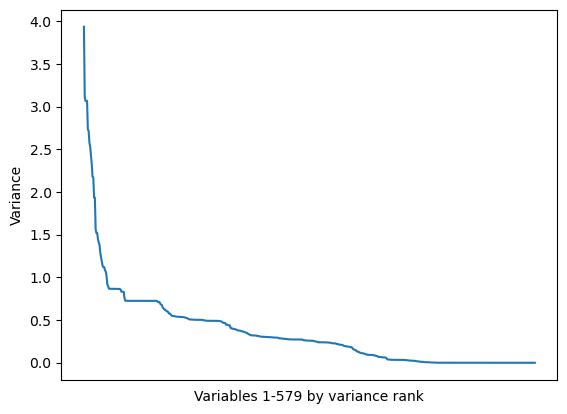
\includegraphics[width=\columnwidth]{Figures/Graphs/Total_variance}
\caption{Scaled variance of all the variables}
\label{variance}
\end{figure}

\subsection{Variable vs feature}
In time series learning, the terms variable and feature are often used interchangeably, which can cause confusion. 
Crucially, variables are a type of feature. 